\documentclass[tikz,border=8pt]{standalone}
\usepackage[utf8]{inputenc}
\usepackage[OT4,plmath]{polski}
\usepackage{amsmath}
\begin{document}
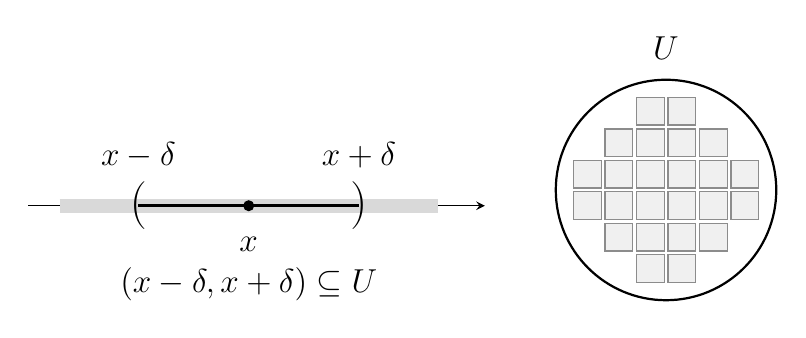
\begin{tikzpicture}[font=\large,>=stealth]
  \draw[->] (0,0)--(5.8,0);
  \draw[line width=5pt,black!15] (.4,0)--(5.2,0);
  \draw[very thick] (1.4,0)--(4.2,0);
  \node[font=\LARGE] at (1.4,0) {$(\vphantom{x}$};
  \node[font=\LARGE] at (4.2,0) {$)\vphantom{x}$};
  \fill (2.8,0) circle (2pt);
  \node[below=8pt] at (2.8,0) {$x$};
  \node[above=10pt] at (1.4,0) {$x-\delta$};
  \node[above=10pt] at (4.2,0) {$x+\delta$};
  \node at (2.8,-1) {$(x-\delta,x+\delta)\subseteq U$};
  \begin{scope}[shift={(8.1,.2)}]
    \foreach \i in {-3,...,2} {
      \foreach \j in {-3,...,2} {
        \pgfmathtruncatemacro{\inside}{
          max(abs(\i*.4),abs((\i+1)*.4))^2+
          max(abs(\j*.4),abs((\j+1)*.4))^2<1.9 ? 1 : 0}
        \ifnum\inside=1
          \draw[black!45,fill=black!6]
            ({\i*.4+.025},{\j*.4+.025})
            rectangle ({(\i+1)*.4-.025},{(\j+1)*.4-.025});
        \fi
      }
    }
    \draw[thick] (0,0) circle (1.4);
    \node at (0,1.8) {$U$};
  \end{scope}
\end{tikzpicture}
\end{document}
